\documentclass{article}    

\usepackage{graphicx}		
\usepackage{hyperref}

\makeatletter
\newcommand\HUGE{\@setfontsize\Huge{50}{60}}
\makeatother

\begin{document}        


\thispagestyle{empty}
\begin{center}
\begin{minipage}{0.9\linewidth}
\flushright
	      		 
    
\includegraphics[width=0.5\linewidth]{univie.jpg}\par
    \vspace{1.5cm}
\centering 	

	{\scshape{\HUGE Bachelor Thesis\par}}
	\vspace{1cm}

    {\scshape{\Large Evaluating Data Management Patterns in Microservice-Based Applications \par}}
    \vspace{2cm}
    
  
 Author  \linebreak
 {\Large  Eylül Gökce Harputluoglu \par}
 	\vspace{1.5cm}
desired academic degree \linebreak
 {\Large Bachelor of Science (BSc)\par}
	\vspace{1.5cm}

\flushleft
	

\begin{tabular}{ll}
Vienna, 01.02.2021	\linebreak
\vspace{1cm}&   \\
  Student ID: & A11728483 \vspace{0.3cm} \\ 
  Subject Area: & Computer Science  -  Medical Informatics \vspace{0.3cm} \\
  Supervisors: & Univ.-Prof. Dr. Uwe Zdun \vspace{0.3cm} \\
  & BSc MSc  Evangelos Ntentos \\
 \end{tabular}


    
    
\end{minipage}
\end{center}
\clearpage

\pagebreak


\section*{Acknowledgements}
Evangelos Ntentos gave me valuable guidance through the project. I would like to thank Mr. Ntentos for providing useful reading materials and for supporting the design of all the patterns by giving beneficial feedback. I also would like to thank Professor Dr. Uwe Zdun for giving me an opportunity to do this project in the Software Architecture Research Group. I would like to thank my sister Hande Harputluoglu as well for the motivational support during this project.  
\clearpage

\tableofcontents

\pagebreak


\section{Microservices}

Microservices is an architectural and organizational approach to software development where an application consists of small independent or loosely-coupled services that communicate over well-defined APIs\cite{amazon}. They can be implemented by using different programming languages, databases, hardware and software environments, depending on what fits best for its purpose\cite{intro}. These services are owned by small teams and are maintainable and testable. Microservices architectures allow applications to be developed faster and scaled easier\cite{intro}. Microservices are used widely by certain software companies such as Amazon, Netflix, Ebay, Uber and more.   

\subsection{Monolithic vs. Microservices Architecture}

With monolithic architectures, processes are not independent and they run as a single service\cite{amazon}. If there is a problem in one process, entire architecture may be affected or changed. With time, the code becomes increasingly complex, and adding new features or updating the existing ones starts costing too much time and effort\cite{mono}.
\bigbreak

\noindent In microservices, adding or improving features is easier. They are built for business capabilities and each service performs a single function. Services are independent from each other and they can be updated, changed, or scaled depending on the needs of the service\cite{amazon, book}.

\subsection{Benefits of Microservices Architecture}

Microservices have the following features which are important and beneficial in software development\cite{intro2}:

\begin{itemize}
    \item With microservices architectures, an application is easier to understand, develop and test.
    \item Each service is owned by a small team. As services are function-specific and independent of each other, teams can focus on only one service and work more quickly, thus the development cycle time gets shorter.  
    \item Microservices allow each service to be independently scaled and to maintain availability when a service experiences a high demand.
	\item Microservices facilitate continues integration, continuous delivery and deployment \cite{wiki}. It makes it easier to try out new ideas and reverse them if they don’t work as expected.
	\item For each service, teams are free to choose the best tools to solve their specific problems without following a strict procedure or any design patterns. Each service can use its own language, framework etc.
	\item Each service is responsible for one function, thus it enables teams to use functions for multiple purposes. 
	\item In microservices, application’s failure is less probable. In a monolithic architecture, if a single component fails it can cause the entire application to fail which is not the case with microservices. Additionally, as microservices make it easier to debug and test applications, the probability to have an error-free application is improved\cite{cio}.

\end{itemize}

\subsection{Goal of the Project}
The goal of this project is to implement a web shop application based on microservices. Three data management patterns will be used in implementation and three prototypes will be created by using the corresponding patterns. The prototypes will be tested in different scenarios and their performances will be compared. The objective of this project is to understand data management patterns and their use in microservices design. At the end of this project, it is expected to see the impact of structural patterns on the performance of application.
\pagebreak

\section{Related Work}

Today many service-based systems follow the microservice architecture model. Microservice architecture is usually used to build distributed systems and to have independent service development and loosely coupled dependencies between services. There are many microservice and data management patterns and the most suitable one can be chosen depending on the system properties\cite{uni}.
\bigbreak
\noindent Besides the patterns used in this project, there are more patterns which can be implemented for the microservice architecture, such as decomposition patterns, additional data management patterns, messaging and remote procedure invocation patterns, deployment patterns, different patterns for communication style, UI patterns, observability patterns, access token, circuit breaker, testing patterns, cross-cutting concerns patterns and many more\cite{io}. 

\subsection[Example of Microservices Based Application: Amazon]{Example of Microservices Based Application: \\ Amazon}

Amazon is a technology company which focuses on e-commerce, cloud computing, digital streaming and artificial intelligence. It started as an online marketplace for books but later expanded to selling electronics, software, video games, etc\cite{wiki}.
\bigbreak
\noindent Amazon is one the first companies which transformed its system into microservices. Previously, Amazon’s architecture was considered as a monolith since all the components in the system were tightly coupled. As most of the companies did, Amazon took a monolith-first approach in its early days since it was a very quick way to start. However, as the company grew bigger, there were more developers working on various projects which made the code larger and the architecture became complex.\cite{amazon1} To be able to change a feature, the whole system needed to be rebuilt and the test cases needed to be rerun. Major code changes were awaited in the deployment pipeline for weeks before the customers could use them.\cite{amazon2} Therefore, there was a need to separate the services so that the software development life cycle is expedited.  To solve these problems, they had a principle which dictates that each function should have a single purpose and they could only communicate through their own APIs. This is also the main principle behind microservices architecture. Breaking down structures into single applications allowed developers to see where the bottlenecks are, therefore shortening the pipeline. Moving to the Amazon Web Services (AWS) cloud allowed Amazon to scale up or down when necessary, reduce the number and duration of outages, and save money\cite{amazon3}.

\pagebreak


\section{Patterns} \label{Patterns}

In order to evaluate and compare the performance of the microservice-based applications, there are three different data management patterns which are implemented in this bachelor project. These patterns are database per service, shared database for all services and an event-based communication between services. 

\subsection{Database per Service}

The database per service model supports the idea that it should keep each microservice’s persistent data private to that service and this data should be accessible only via its API. A service’s database is part of the service implementation; therefore it cannot be accessed by other services. In this model, a service’s transactions involve only its database\cite{microserviceDB}. 
\bigbreak

\noindent Using a database per service pattern has several benefits:

\begin{itemize}
    \item The services are loosely coupled which means that each of its components has little or no knowledge about other components. If there is a problem or a change in one of the databases, the other services won’t be affected by that.
    \item Each service can use a specific type of database which is appropriate to its needs and functions. 
\end{itemize}

\noindent Using a database per service has also a few drawbacks\cite{microserviceDB}:

\begin{itemize}
    \item 	Some data can exist in multiple databases and since these databases are independent and can be in form of different types, it is challenging to implement queries which use these shared data. 
    \item	Managing multiple SQL and NoSQL databases is complex.
    \item	Implementing business transactions that extend to multiple services is not straightforward.
\end{itemize}

\noindent While using this pattern in this project, problems due to these drawbacks were faced in the implementation, especially where it was necessary to use a join operation between different service databases.  
 

\subsection{Shared Database}

The second database architecture used in the implementation is shared database. The idea behind this architectural design is that each service freely accesses data owned by the other services by using local ACID (atomicity, consistency, isolation, durability) transactions\cite{microserviceSharedDB}. All services are using the same database in the system. 

\bigbreak
\noindent This pattern has following benefits in the microservice-based applications\cite{microserviceSharedDB}:

\begin{itemize}
    \item 	A developer uses familiar and straightforward ACID transactions to ensure data consistency.
    \item	A single database is simpler to work on.
\end{itemize}

\noindent A shared database for the microservices has also few drawbacks\cite{microserviceSharedDB, mic}:

\begin{itemize}
    \item 	There is a requirement for development time coupling to ensure data consistency:  A developer works on one service and this service needs to coordinate schema changes with the developers of other services that access the same tables. This coupling and additional coordination will slow down the development process.
    \item There is a requirement for runtime coupling. Since all services access the same database, they can potentially interfere with one another. For example, if long running service transaction holds a lock on one table in the database, then the other services which need to access this table will be blocked until long running service transaction releases the lock. Otherwise, there will be inconsistency between table content which can cause problems.
    \item Single database might not satisfy the data storage and access requirements to this database from different services may be different.
    \item In shared databases, it is harder to extend the application with new services. 
\end{itemize}

\noindent In order to support ACID principle and to avoid possible problems, database transaction method  was implemented inside of the Order Service to make an order disposable.  

\subsection[Event-Based Communication: Message Broker Pattern]{Event-Based Communication: Message Broker \\ Pattern}

The previous patterns were based on synchronous communication with using REST API (REpresentational State Transfer) between services which means the client forwards a REST request and actively waits for a response.  Generally, in synchronous communication, the client prepares the message and transmits it over the network to the server. It waits for a response and while waiting it does not perform any other processing as part of its computing thread\cite{microserviceEventBased2}.  
\linebreak

\noindent As the third pattern, an event-based communication between microservices has been chosen. In order to realize an event-based communication, message broker pattern was used in the implementation of this project. This model connects microservices through the transmission of messages while using a broker. A microservice publishes an event when something notable happens, such as when it updates a business entity. Other microservices subscribe to those events and are notified when there is a change in these events. When a microservice receives an event, it can update its own business entities accordingly. This update may lead to more events being published. This is the essence of the eventual consistency concept. This publish/subscribe system is usually performed by using an event bus. The event bus can be designed as an interface with the API to subscribe and unsubscribe to the events and publish events\cite{microserviceEventBased, microserviceEventBased3, microserviceEventBased4}.
\linebreak

\noindent Thanks to this pattern, the asynchronous communication can be built between services that the client can send a message/request, but he does not have to wait for a response. 
\bigbreak
\noindent This model has the following benefits \cite{microserviceEventBased4, microserviceEventBased2}:

\begin{itemize}
    \item The components may have different models of communication. With the Message Broker, communication between the components is supported and possible. Message queue, request-response mode, broadcast mode are examples of good use of Message Broker with different models of communications.
    \item Message Broker Pattern supports different message formats like JSON, Protobuf etc.
    \item The broker communication approach is ideal for one-way calls: sending message and not waiting for the response.  It helps to balance the load on individual layers of the system and thus supports peak demands in an inbound traffic.
    \item There is no risk of overloading the message consumers.
    \item This pattern also allows you to save messages permanently for a better reliability, or only process them in memory for better efficiency.
\end{itemize}

\noindent Using a message broker has also several disadvantages\cite{microserviceEventBased2}:
\begin{itemize}
    \item Modelling the application using messages is more complicated.
    \item One of the message broker technologies should be set up in the system. However as broker is an additional object in the architecture, it is another potential failure point in the system. With broker use, there may be problems related to quorum behaviour, delivery guarantees, idempotency verification etc\cite{microserviceEventBased2}.
    \item There is a possibility of overloading the queues or message broker when the message consumer is not available for a while. 
    \item Message broker introduces delays in communication because broker runs in the memory mode and execution can take some time if the model exists in the disk.      

\end{itemize}

\noindent In this project, RabbitMQ is used in order to build the event-based communication between services.

\section{Case Study}
In this project, there is one microservice-based application idea. A web shop application based on microservices is implemented by using three different patterns. 

\subsection{Technology Stack}
All three patterns are implemented with using C\# programming language. Therefore, the .Net Core framework is used for the microservice implementation. For the API gateway, Ocelot is used for the .Net Core application. The databases of all microservices are created in MySQL Database. For the third pattern (message broker pattern), an additional technology named RabbitMQ is used. For testing the applications, Apache JMeter is used. 

\subsection{Description: Web Shop}
The main application idea of this project is building a web shop, where the customer of the online shop is the client. A web shop requires a customer service, a product service, a cart service, an order service, a payment service and a notification service. These services are implemented with microservices. The client can easily register to the system, select a product, add it to the cart and order cart. At the end, he virtually pays the total amount of the products from his cart. The customer receives notifications about errors as well as information messages.  

\subsubsection{Customer Service}
The customer service is designed for handling the customer information by only connecting to the customer database. In the customer service, either a new customer is registered to the system, or customer id  is found by using customer information.

\subsubsection{Product Service}
The product service is designed for handling all the products and their quantities in the storage. Inside of this service, it is possible to list all the products and their information, select a product and if the product is sold, update the quantity in the database. 

\subsubsection{Cart Service}
The cart service does not use an actual database nevertheless it saves customer IDs and all carts belonging to the customers. Customers can insert new products to their cart, and when they go to their cart, all the selected products are listed. 

\subsubsection{Order Service}
The order service is the most complicated service in the whole application. The client can order the entire cart where different products with different quantities are listed. Once a new order is created, the service gets all the products and calculates the total price. To be able to calculate the total price, order service finds products’ prices by using their product ID and it simply multiples products’ prices with desired number of units and adds them together. It updates the product database with the quantities of product which will change after the purchase and finally saves all products and the total price with this order ID. To avoid any possible problems while doing all these processes, the database transaction method is used in the implementation. The client can get all of its orders or get all products by giving an order ID. 

\subsubsection{Payment Service}
The payment service is responsible of the payment of the total amount for the order. We can insert a payment inside of this service and after the order is paid, the payment is saved to the database. It is also possible to list all previous payments inside of the payment service.

\subsubsection{Notification Service}
Notification service has three principle functions: adding a new notification, dismissing the current notification and listing all the notifications. All other services are using notification services to send a notification to the client. In this system, it is possible to get errors. These errors can appear because of an inconsistent input or data which will throw exceptions in the implementation or they can be HTTP-REST errors. Notification service gets errors, which are originated in this service or in the other services. It translates errors in a human-readable manner so that clients can read and understand the notifications.
\linebreak 
\linebreak
For example,  a customer tries to buy a product with 100 units but there are not enough units in the storage. Therefore, an error appears in product service which is later directed to notification service. Notification service gives a notification to the client about this insufficient units for the desired product. Notification service does not only send notification about the errors but also about acknowledgement and updates. If the customer orders the products and executes the payment without any problem, then the service notifies the customer with an information message about the success of the order.


\subsection{Prototypes}

There are three different patterns described in the previous chapter \ref{Patterns} and in this project, all these patterns are implemented as separate prototypes. 

\subsubsection{Prototype 1: Database per Service}

The first prototype has database per service pattern implementation. Customer service, product service, order service and payment service have their own MySQL databases. For any operations, the services need to access to their databases. In the following figures, a class diagram, a component diagram and a sequence diagram are presented. The original images can be found here: 
\begin{itemize}
    \item \href{https://github.com/eylulgokce/Microservices/blob/main/Thesis/UML%20Diagrams/Class%20Diagrams/microservices_class_diagram.jpg}{Class Diagram for Database per Service}
    \item \href{https://github.com/eylulgokce/Microservices/blob/main/Thesis/UML%20Diagrams/Component%20Diagrams/Comp_Microservice.jpg}{Component Diagram for Database per Service}
    \item \href{https://github.com/eylulgokce/Microservices/blob/main/Thesis/UML%20Diagrams/Sequence%20Diagrams/Sequence_DB.jpg}{Sequence Diagram for Database per Service}
\end{itemize}

\pagebreak

\begin{figure}[h!]
\centering
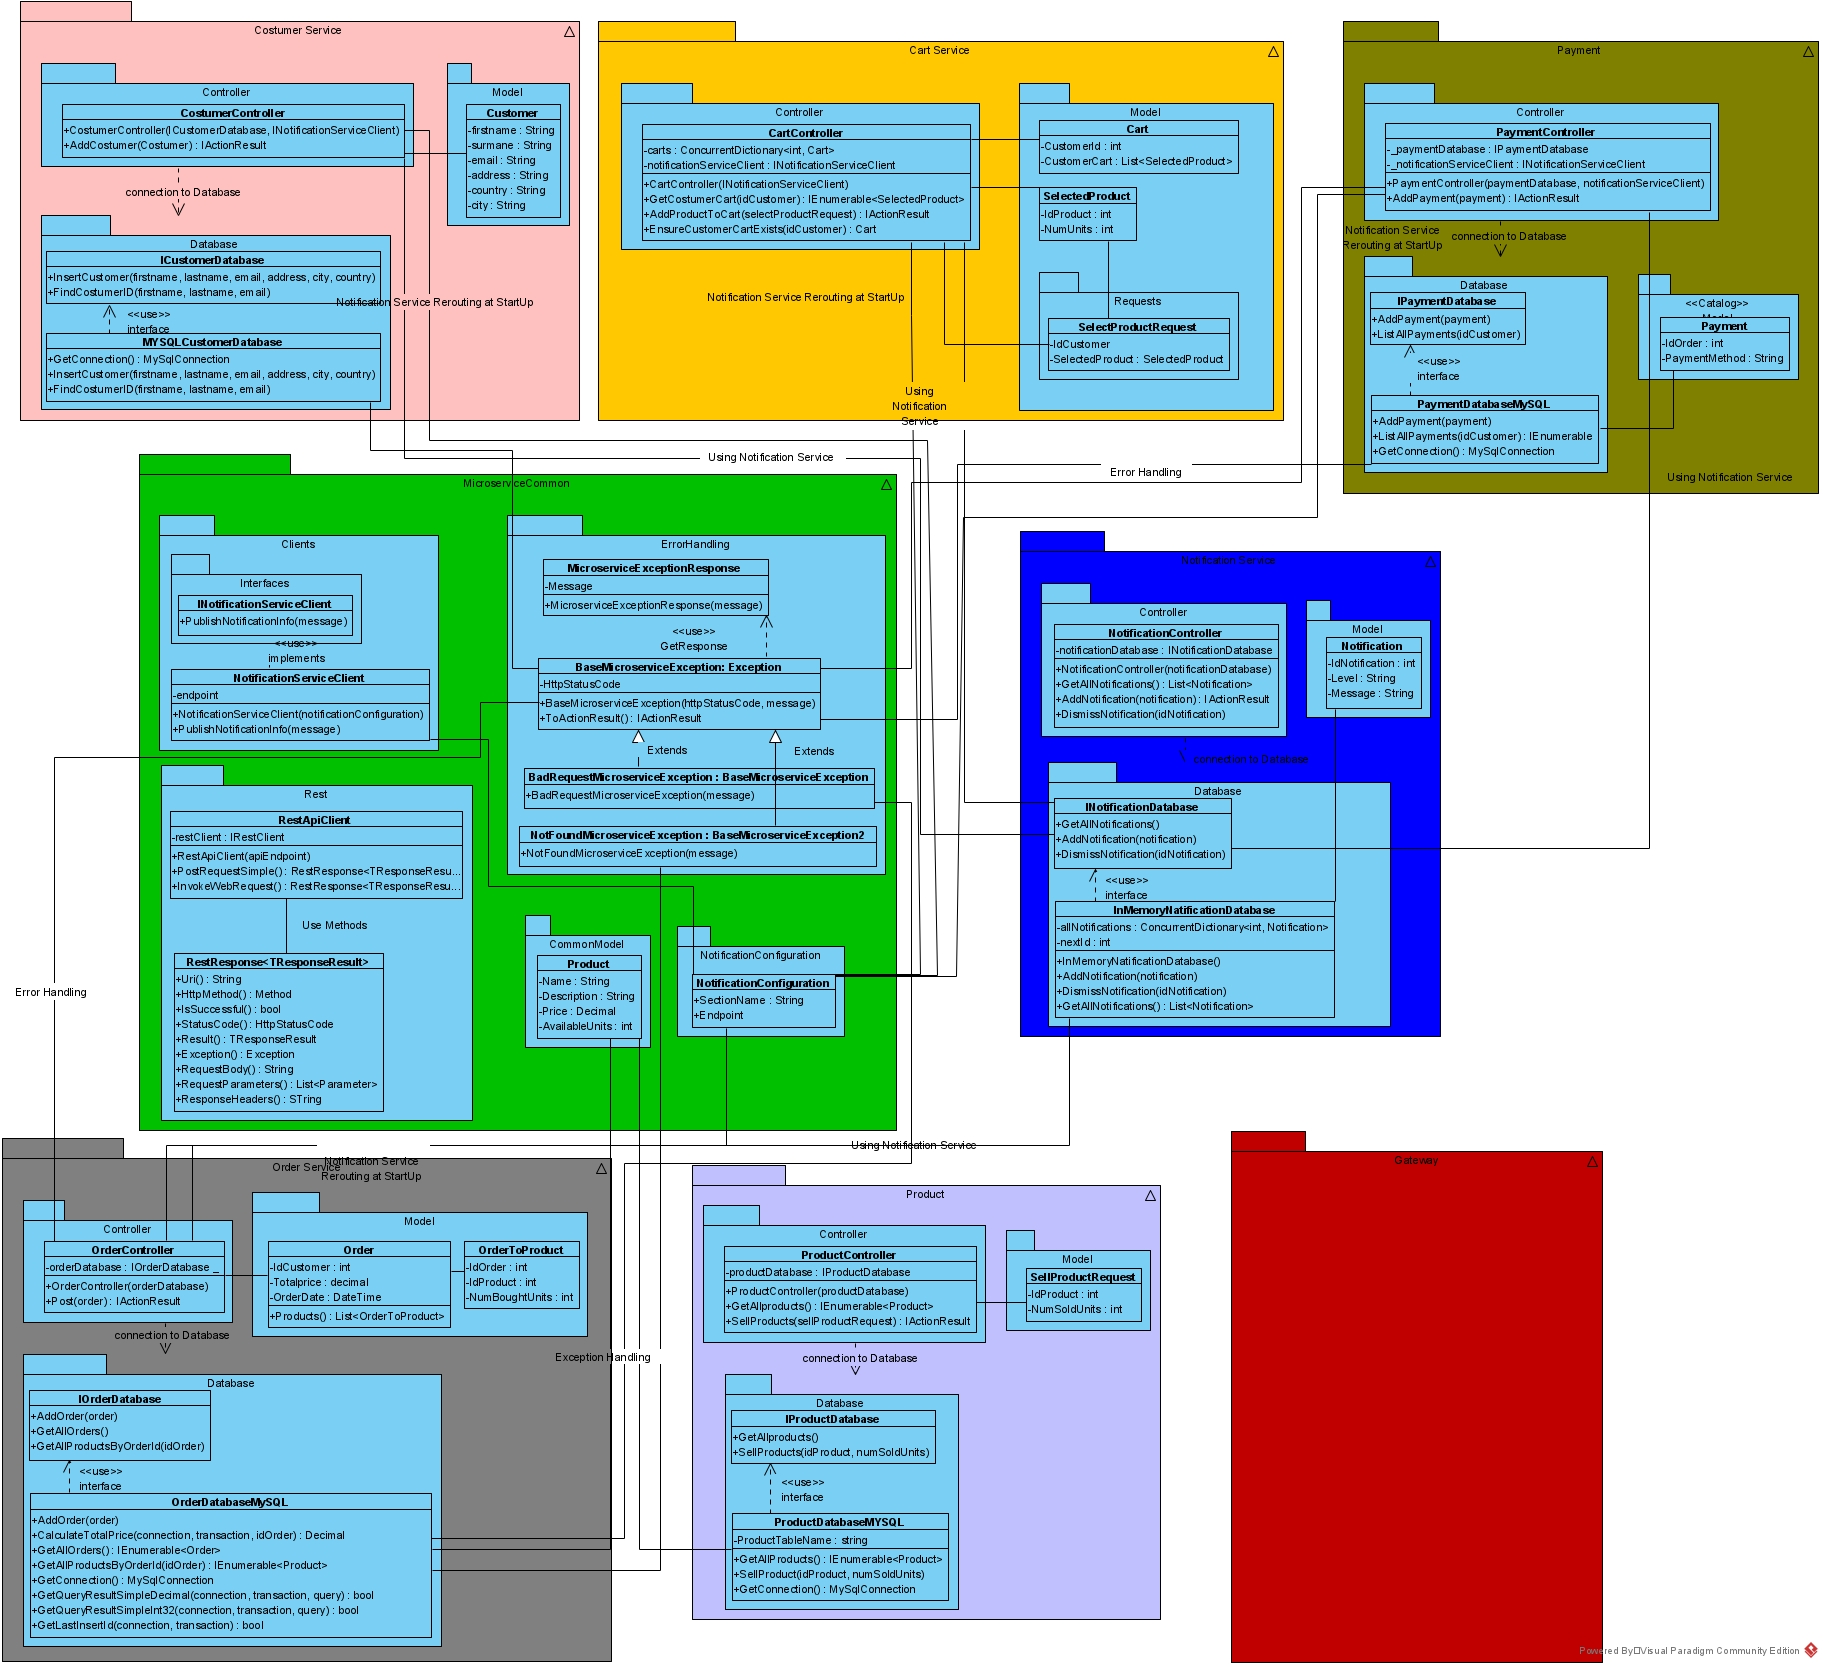
\includegraphics[scale=0.25, angle=90]{class_DB.jpg}
\caption{Class Diagram for Database per Service}
\label{fig:class_DB}
\end{figure}

\pagebreak


\begin{figure}[h!]
\centering
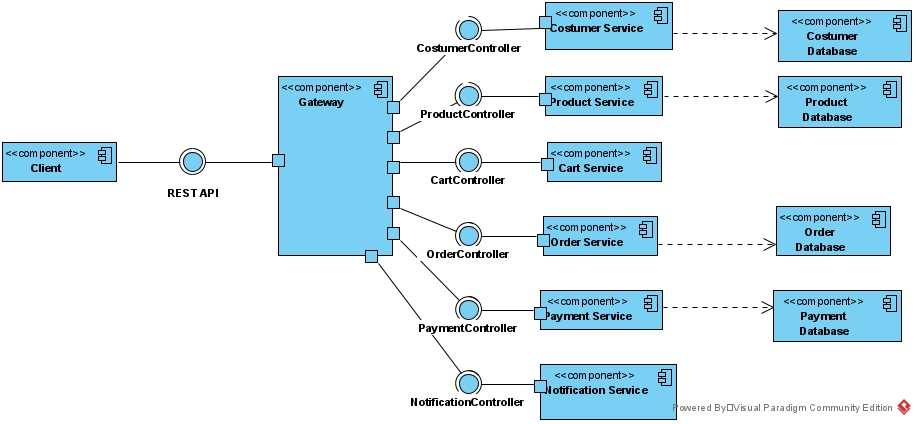
\includegraphics[scale=0.55, angle=90]{Comp_Microservice.jpg}
\caption{Component Diagram for Database per Service}
\label{fig:comp_DB}
\end{figure}

\pagebreak

\begin{figure}[h!]
\centering
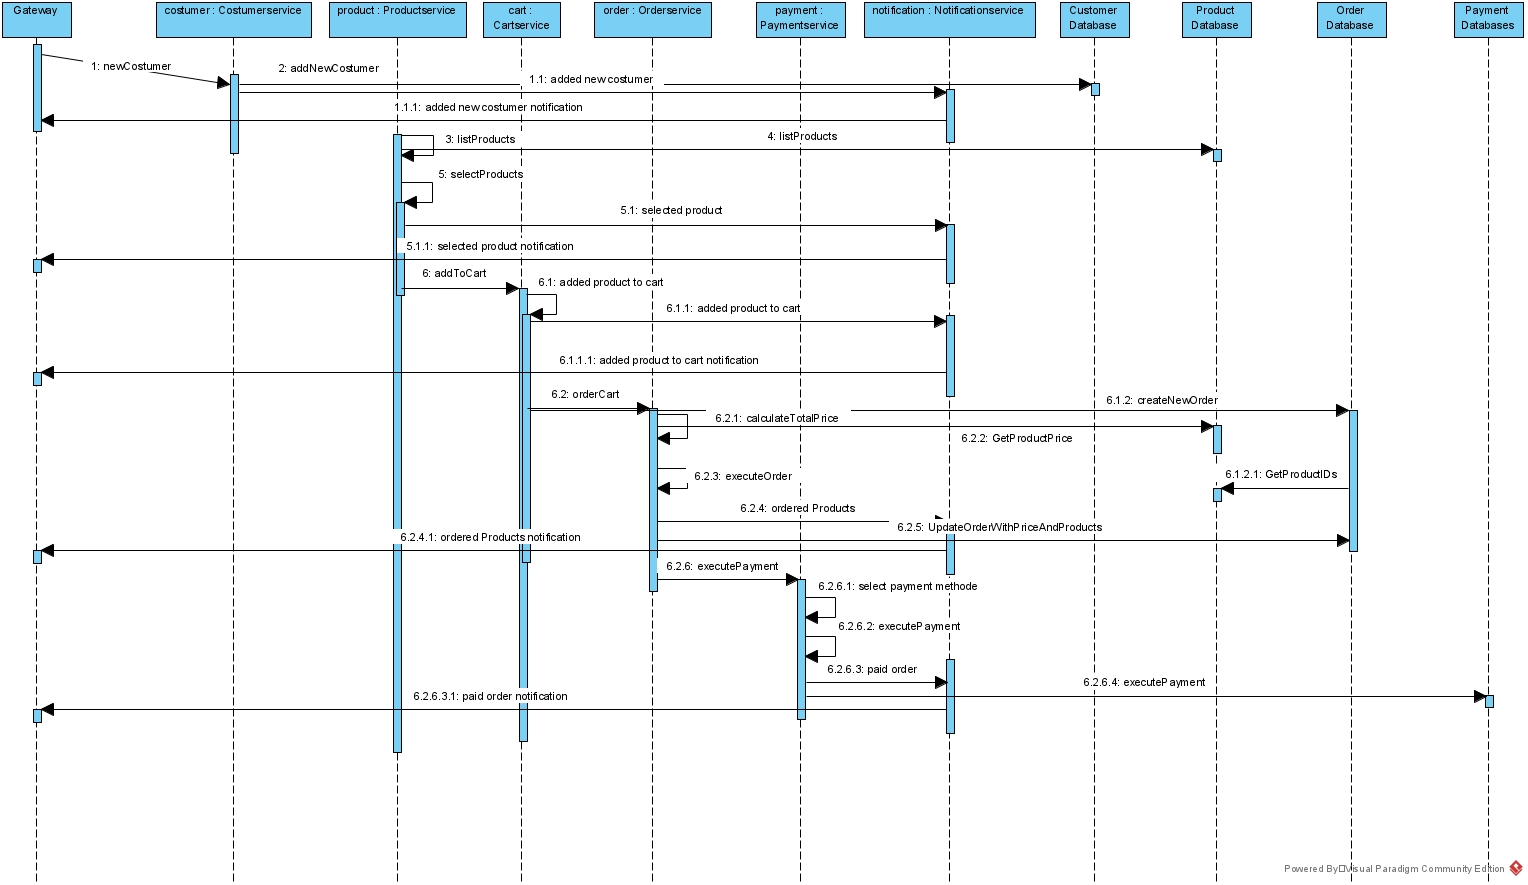
\includegraphics[scale=0.32, angle=90]{Sequence_DB.jpg}
\caption{Sequence Diagram for Database per Service}
\label{fig:seq_DB}
\end{figure}

\pagebreak


\subsubsection{Prototype 2: Shared Database}

The second prototype has a shared database implementation. Customer service, product service, order service and payment service use the same MySQL database. For any operations, the services need to access to a  single database. The rest of the system is same as the first prototype. In the following figures, a class diagram, a component diagram and a sequence diagram are presented. The original images can be found here: 

\begin{itemize}
    \item \href{https://github.com/eylulgokce/Microservices/blob/main/Thesis/UML%20Diagrams/Class%20Diagrams/microservices_class_diagram.jpg}{Class Diagram for Shared Database}
    \item \href{https://github.com/eylulgokce/Microservices/blob/main/Thesis/UML%20Diagrams/Component%20Diagrams/Comp_Shared%20DB.jpg}{Component Diagram for Shared Database}
    \item \href{https://github.com/eylulgokce/Microservices/blob/main/Thesis/UML%20Diagrams/Sequence%20Diagrams/sequence_Shared%20DB.jpg}{Sequence Diagram for Shared Database}
\end{itemize}

\pagebreak

\begin{figure}[h!]
\centering
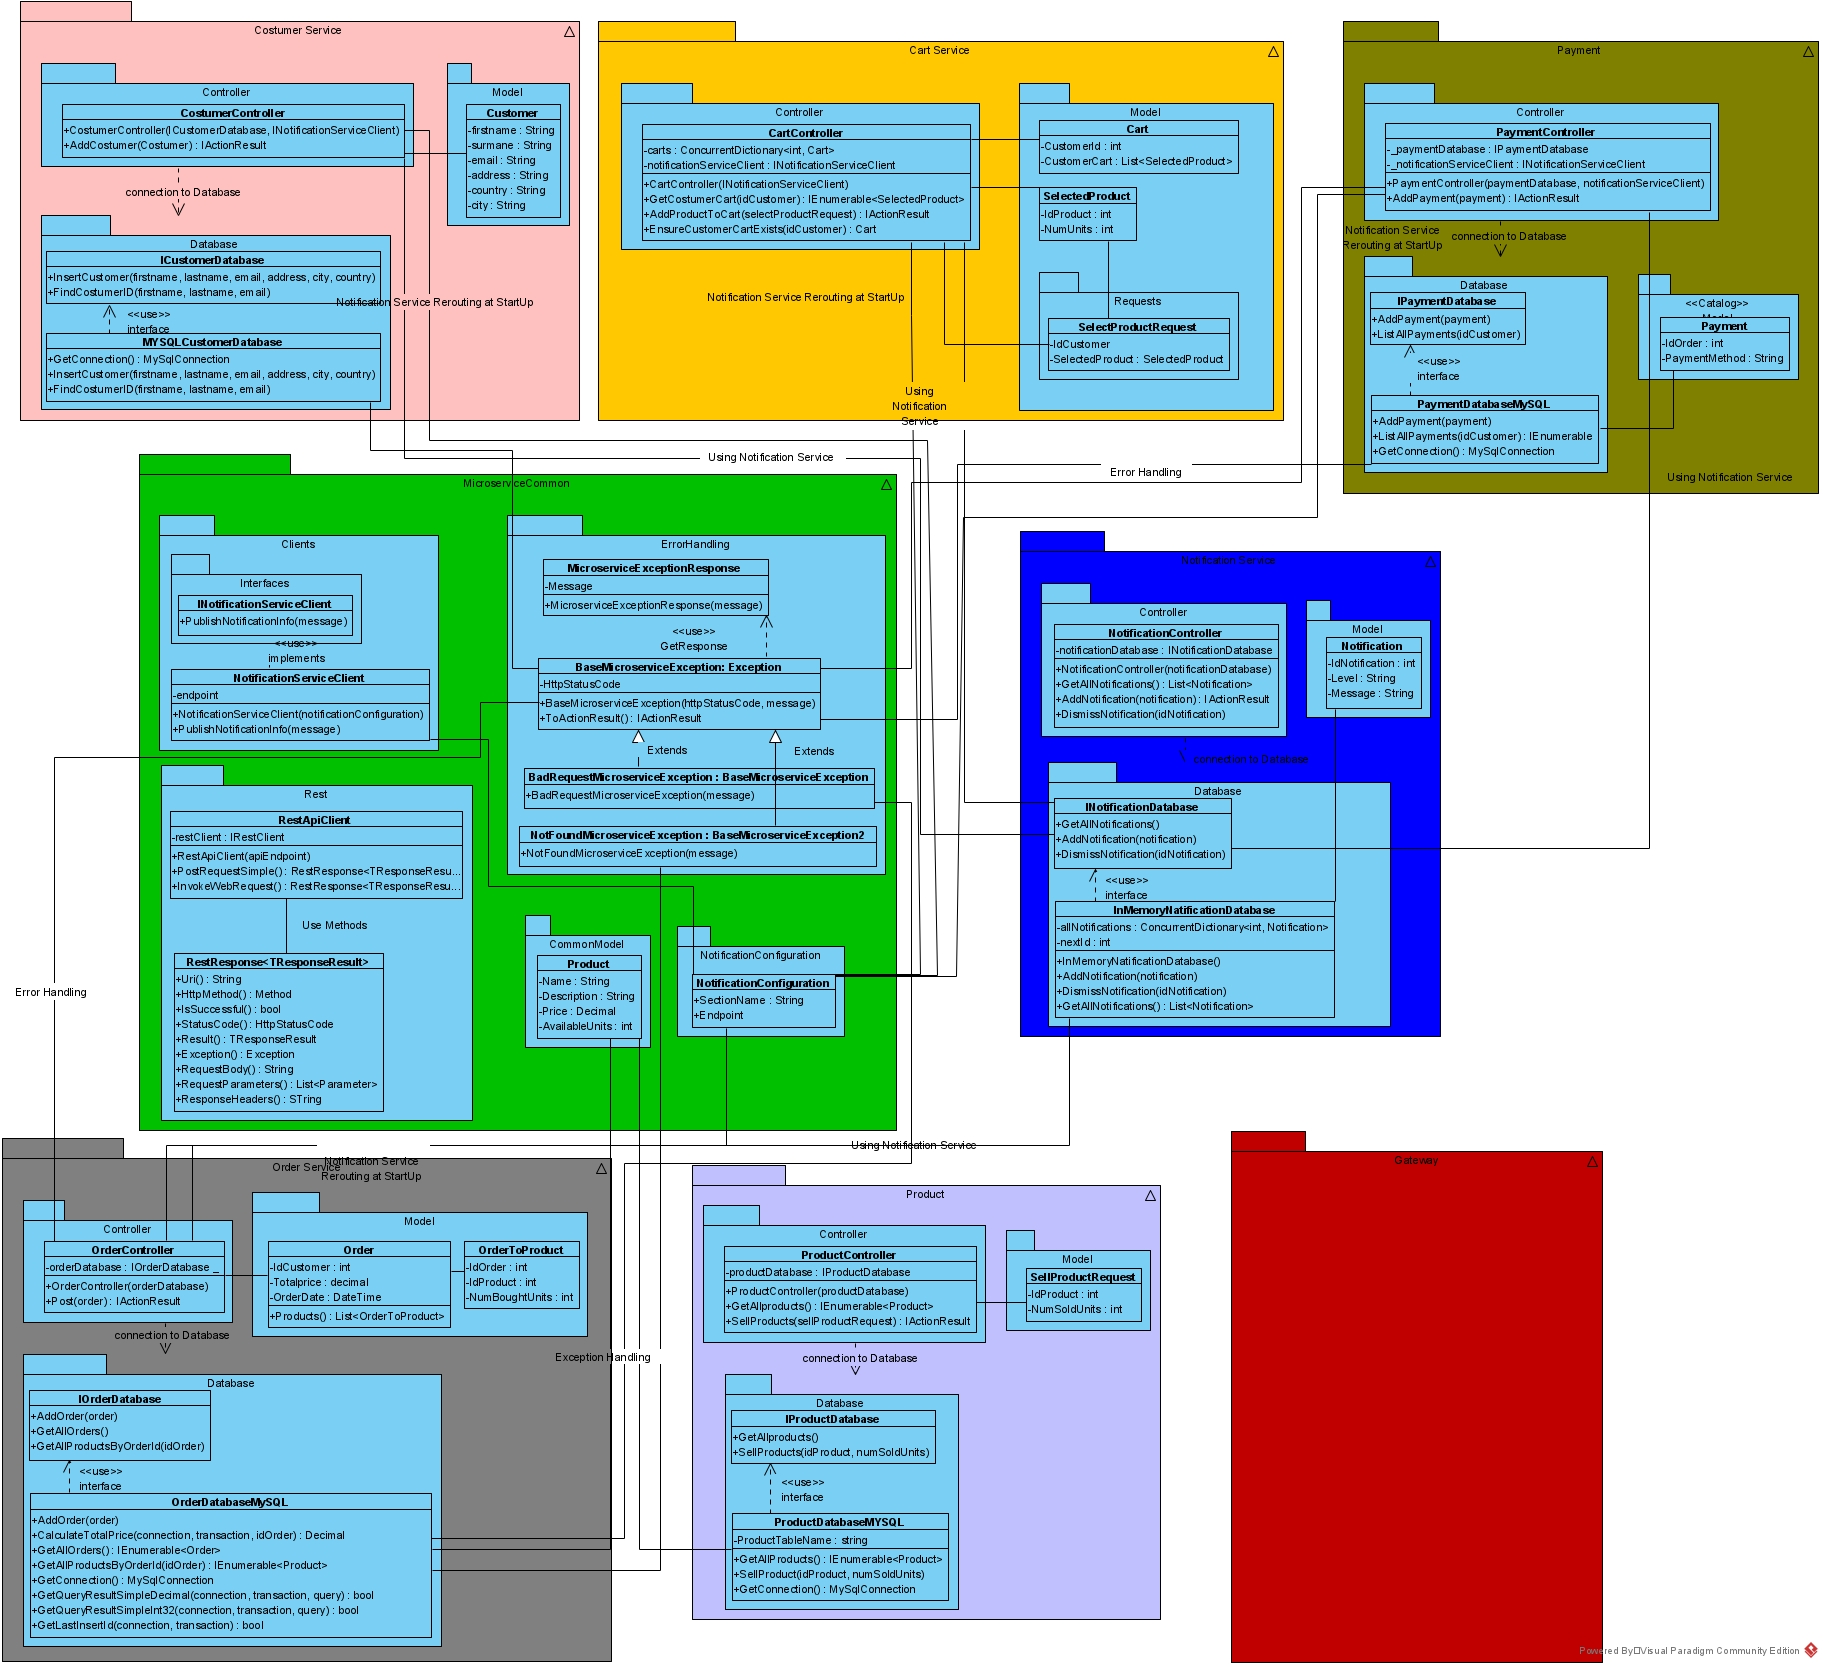
\includegraphics[scale=0.25, angle=90]{class_DB.jpg}
\caption{Class Diagram for Shared Database}
\label{fig:class_shared}
\end{figure}

\pagebreak

\begin{figure}[h!]
\centering
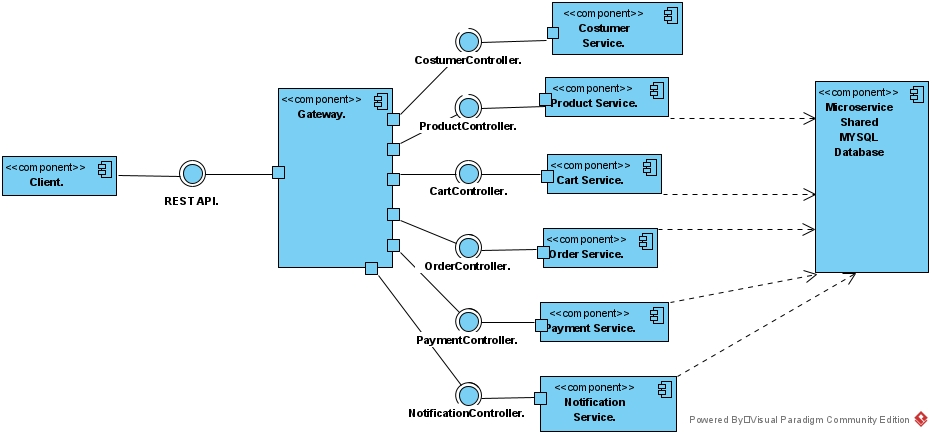
\includegraphics[scale=0.50, angle=90]{Comp_Shared DB.jpg}
\caption{Component Diagram for Shared Database}
\label{fig:comp_shared}
\end{figure}

\pagebreak

\begin{figure}[h!]
\centering
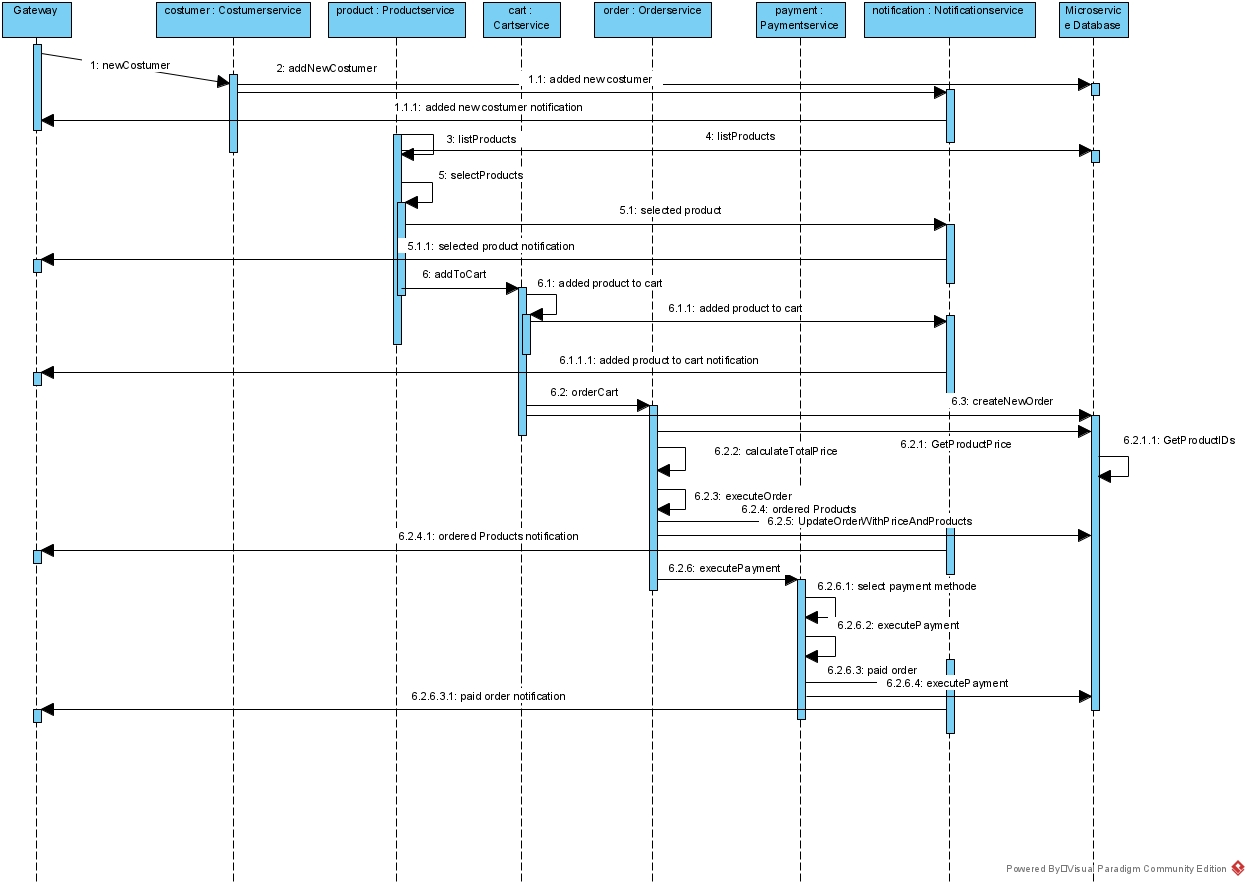
\includegraphics[scale=0.40, angle=90]{sequence_Shared DB.jpg}
\caption{Sequence Diagram for Shared Database}
\label{fig:seq_shared}
\end{figure}

\pagebreak

\subsubsection{Prototype 3: Message Broker}

The third prototype has a event-based communication implementation. The message broker pattern has been implemented in this prototype. Cart service, order service and payment service are part of the communication within message bus. The cart service inserts selected products to the cart and publishes an event. The order service will be activated if the service receives an order. For each order, a payment should be executed. Once the payment service receives a payment, the service will pay the amount of the order. In the following figures, a class diagram, a component diagram and a sequence diagram are presented. The original images can be found here: 

\begin{itemize}
    \item \href{https://github.com/eylulgokce/Microservices/blob/main/Thesis/UML%20Diagrams/Class%20Diagrams/Class%20Diagram%20for%20MessageBroker.jpg}{Class Diagram for Message Broker Patter}
    \item \href{https://github.com/eylulgokce/Microservices/blob/main/Thesis/UML%20Diagrams/Component%20Diagrams/Comp_Message%20Broker.jpg}{Component Diagram for Message Broker Pattern}
    \item \href{https://github.com/eylulgokce/Microservices/blob/main/Thesis/UML%20Diagrams/Sequence%20Diagrams/sequence_Message%20Broker.jpg}{Sequence Diagram for Message Broker Pattern}
\end{itemize}

\pagebreak

\begin{figure}[h!]
\centering
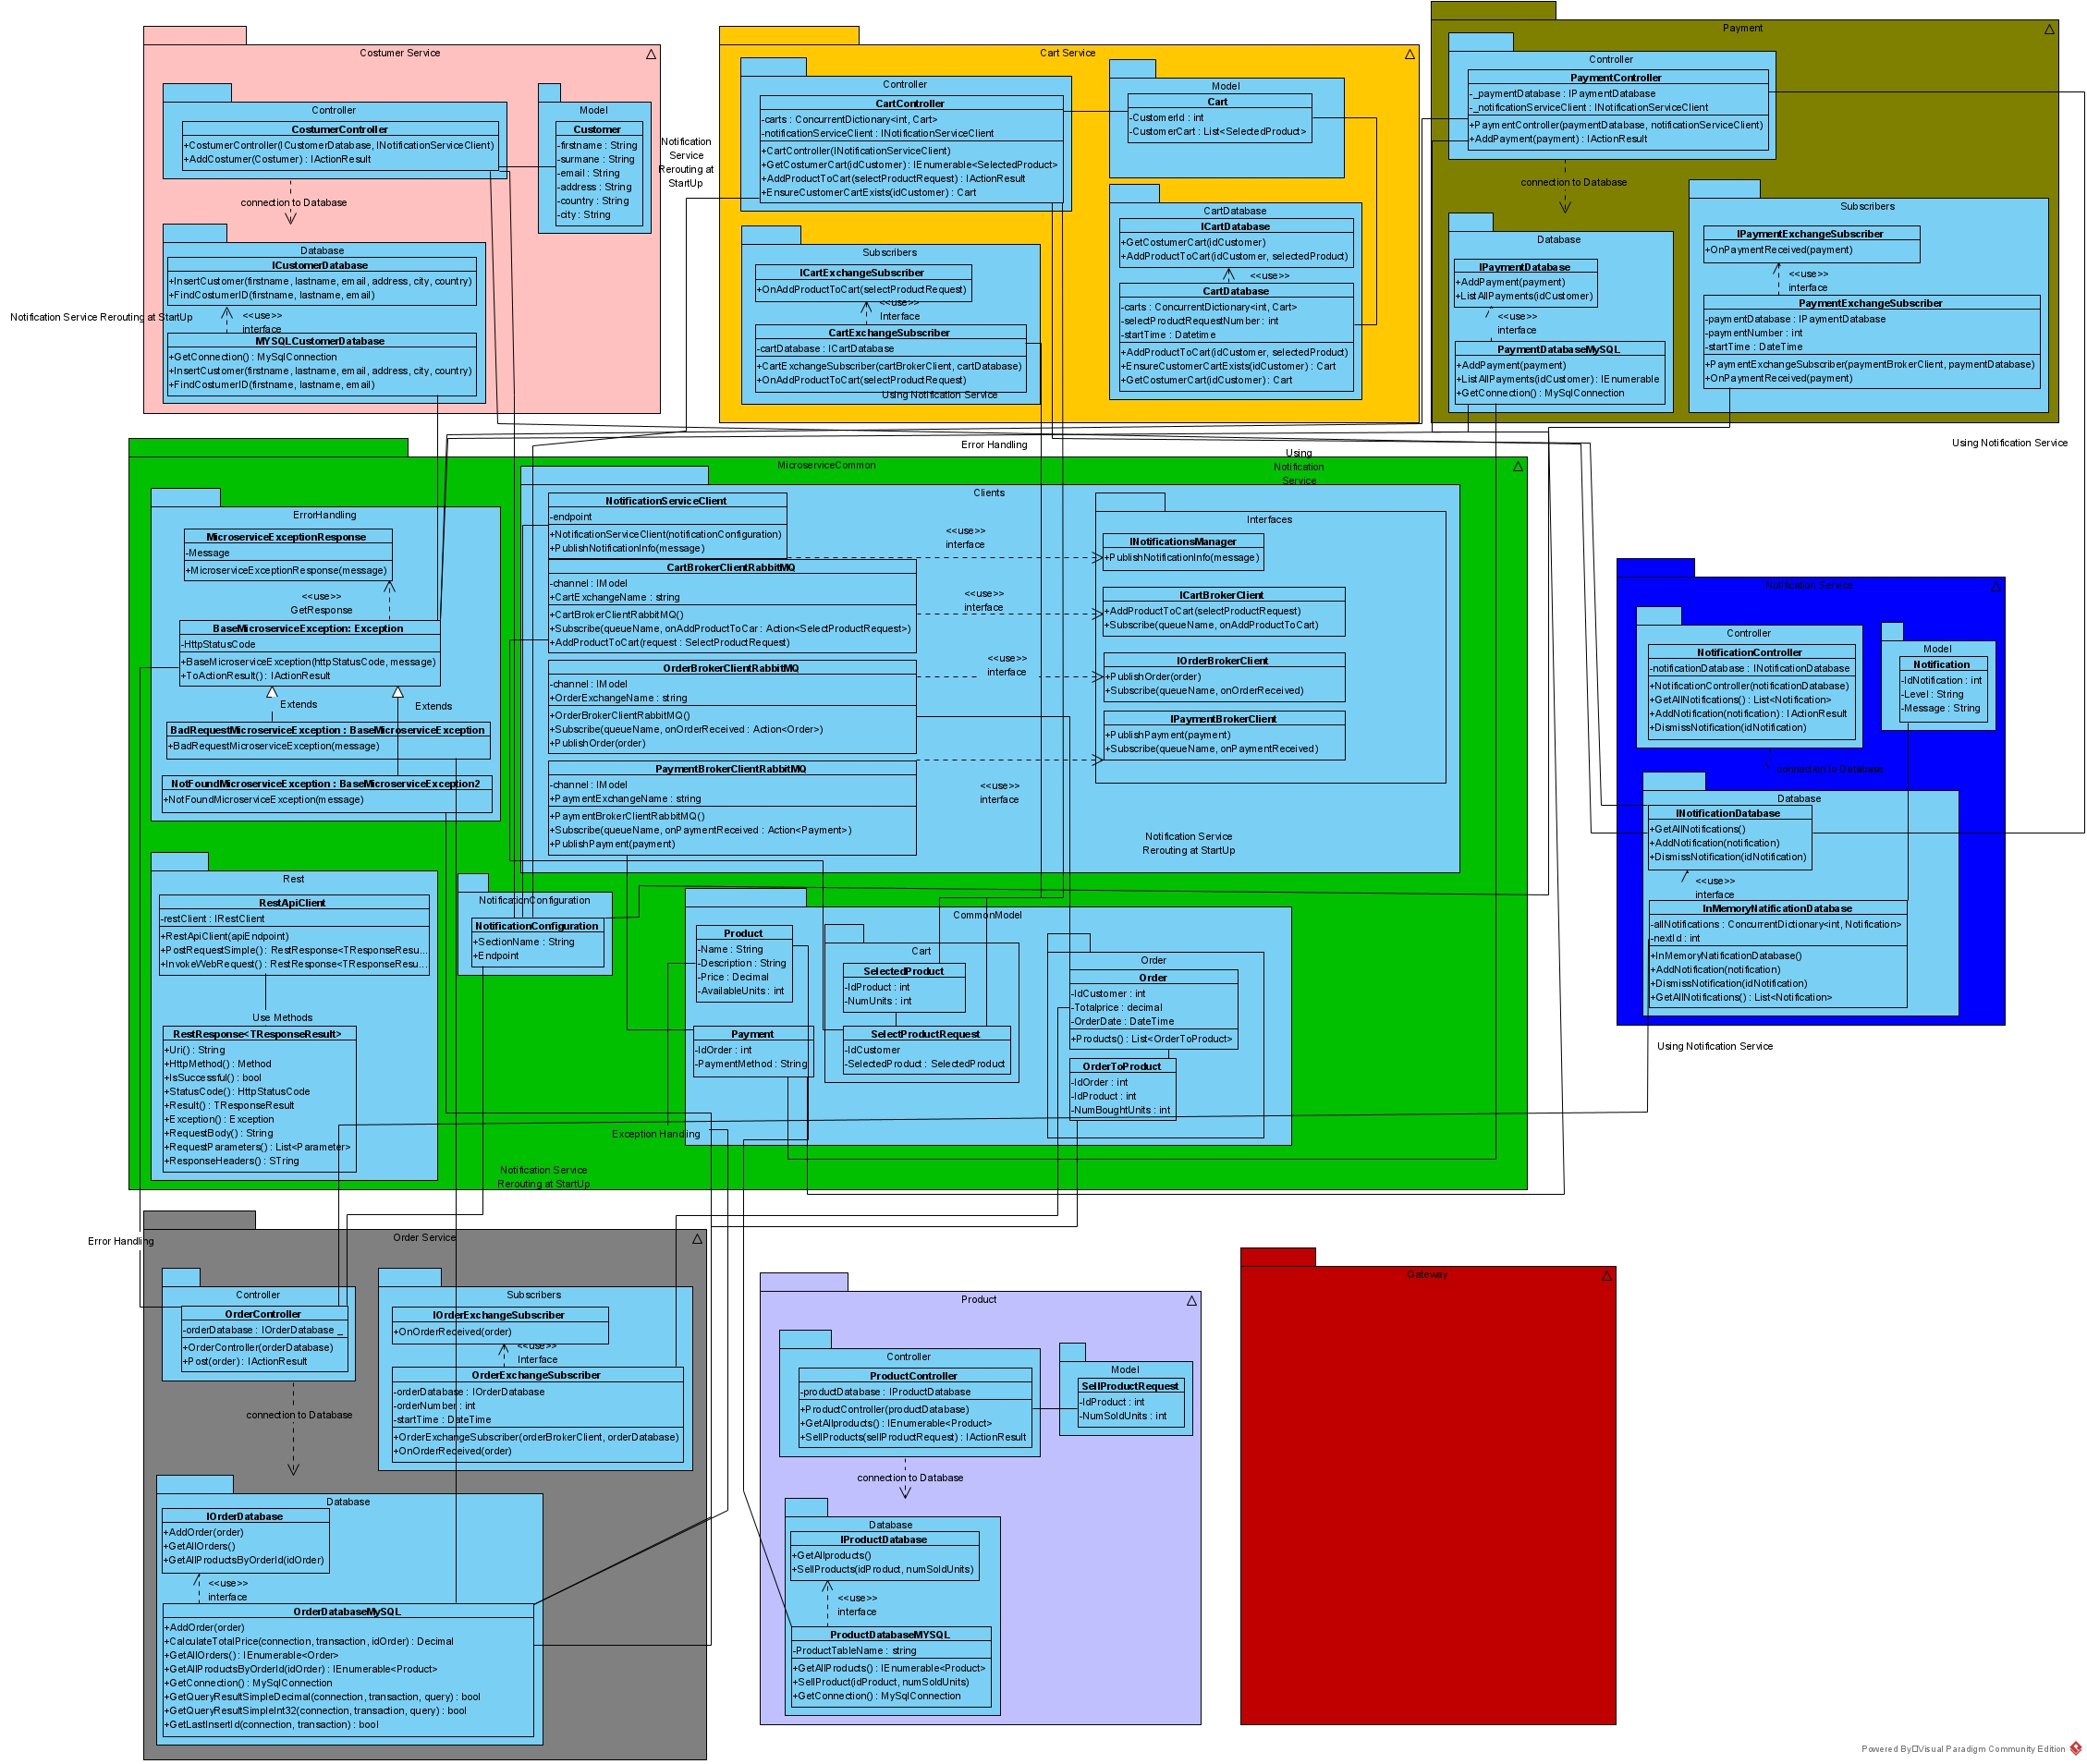
\includegraphics[scale=0.20, angle=90]{Class_MessageBroker.jpg}
\caption{Class Diagram for Message Broker Pattern}
\label{fig:class_broker}
\end{figure}

\pagebreak

\begin{figure}[h!]
\centering
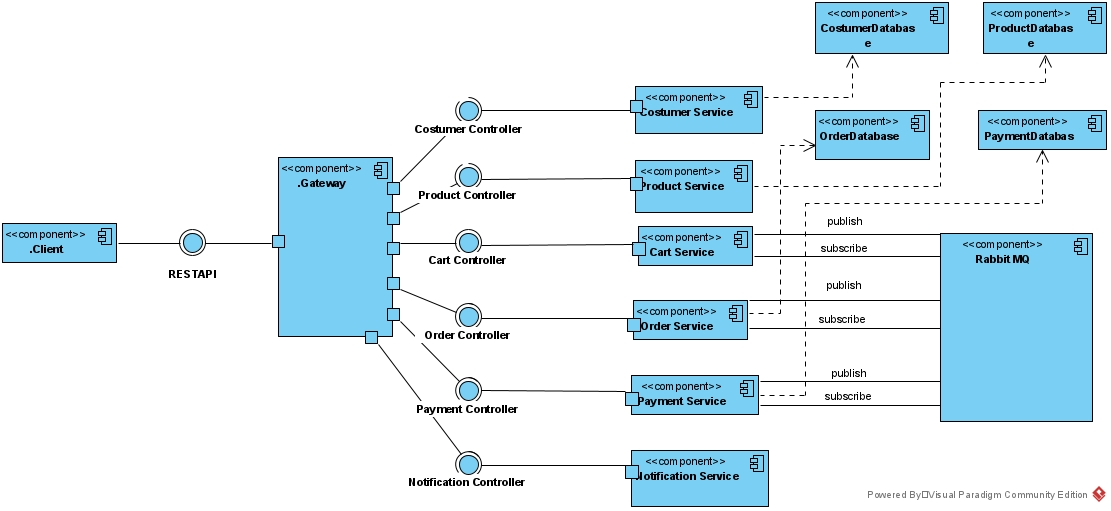
\includegraphics[scale=0.45, angle=90]{Comp_Message Broker.jpg}
\caption{Component Diagram for Message Broker Pattern}
\label{fig:comp_broker}
\end{figure}

\pagebreak

\begin{figure}[h!]
\centering
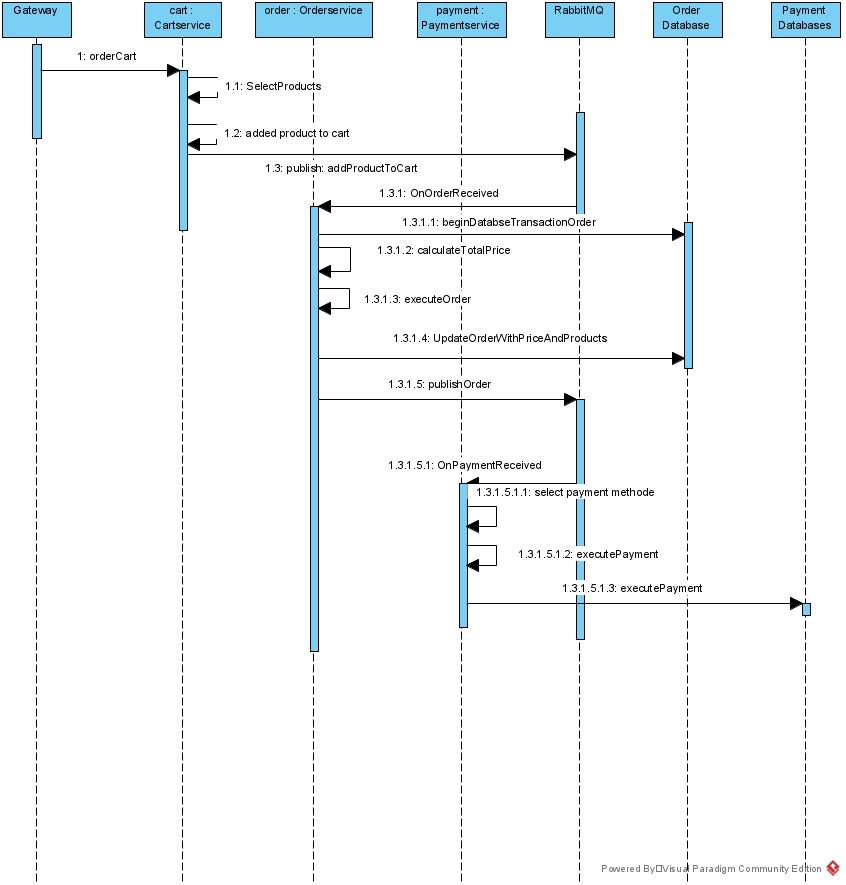
\includegraphics[scale=0.50, angle=90]{sequence_Message Broker.jpg}
\caption{Sequence Diagram for Message Broker Pattern}
\label{fig:seq_broker}
\end{figure}

\pagebreak

\section{Evaluation}

Three prototypes are implemented by using three different patterns: Database per Service Pattern, Shared Database Pattern and Message Broker Pattern. They are tested with different size of samples in different scenarios and test results are analyzed by comparing the performances of all prototypes. Size of sample represents how many times these scenarios have been run randomly and average response time is an indicator of the performance, i.e. shorter average response time corresponding to a better performance.  

\subsection{Test Cases}

There are three different scenarios for the system tests. These tests are implemented in JMeter and they are used for the first and the second prototypes. Part of these scenarios are designed to test the performance of these structural patterns by using REST API.  As Message Broker Pattern does not use REST API for communication commands such as "order products", these scenarios are not suitable for testing the third prototype. To test this prototype, the client is designed manually in C\# and average response time is tracked to measure the performance for different size of samples. 
The sample sizes are 100, 200, 500, 1000 for each prototype testing. The test scenarios for first and second prototypes are the followings:


\begin{itemize}
    \item Scenario 1: 
    \begin{enumerate}
        \item Create Customer
        \item Get All Products
        \item Get Notifications
        \item Add Notifications
        \item Dismiss Notifications
    \end{enumerate}
    \item Scenario 2: 
    \begin{enumerate}
        \item Create Customer
        \item Get All Products
        \item Order Products
        \item Get Notifications
        \item Add Notifications
        \item Dismiss Notifications
    \end{enumerate}
     \item Scenario 3: 
    \begin{enumerate}
        \item Create Customer
        \item Get All Products
        \item Add Product To Cart
        \item Get Customer Cart
        \item Order Products
        \item Get Notifications
        \item Add Notifications
        \item Dismiss Notifications
    \end{enumerate}
\end{itemize}

\bigbreak

\subsection{Results}

The test results are summed up in the following graphs.
\bigbreak

\begin{figure}[h!]
\centering
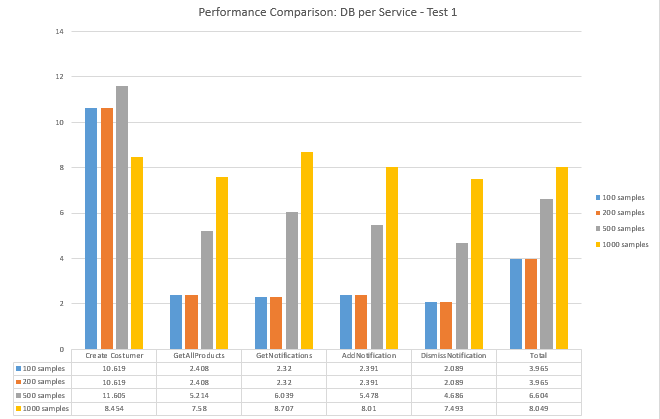
\includegraphics[scale=0.70]{Test_Results/test_1_DB_per_Service.PNG}
\caption{Test 1 - DB per Service}
\label{fig:test_1_DB_per_Service}
\end{figure}

\pagebreak

\begin{figure}[h!]
\centering
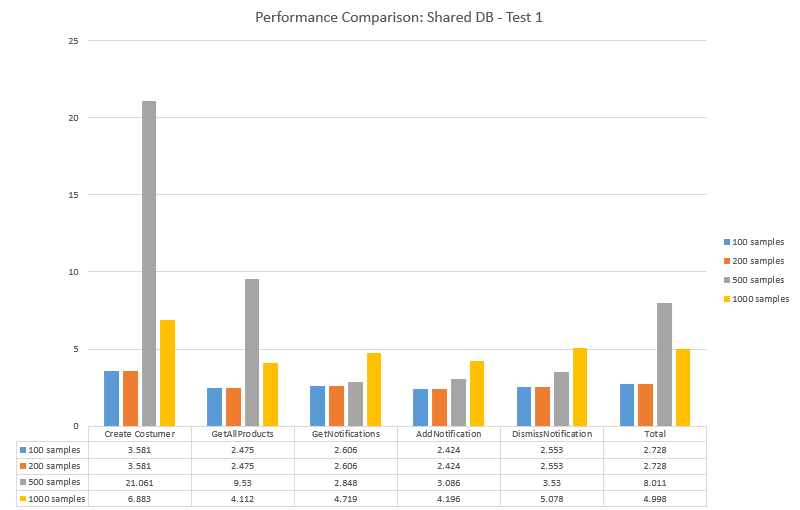
\includegraphics[scale=0.60]{Test_Results/test_1_shared_DB.PNG}
\caption{Test 1 - Shared DB}
\label{fig:test_1_shared_DB}
\end{figure}

\begin{figure}[h!]
\centering
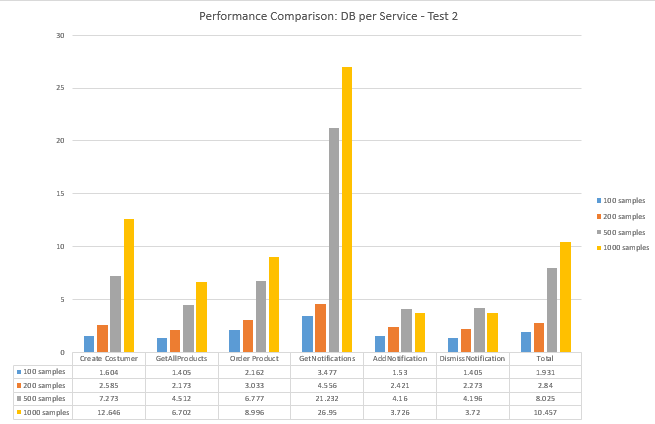
\includegraphics[scale=0.70]{Test_Results/test_2_DB_per_Service.PNG}
\caption{Test 2 - DB per Service}
\label{fig:test_2_DB_per_Service}
\end{figure}

\pagebreak

\begin{figure}[h!]
\centering
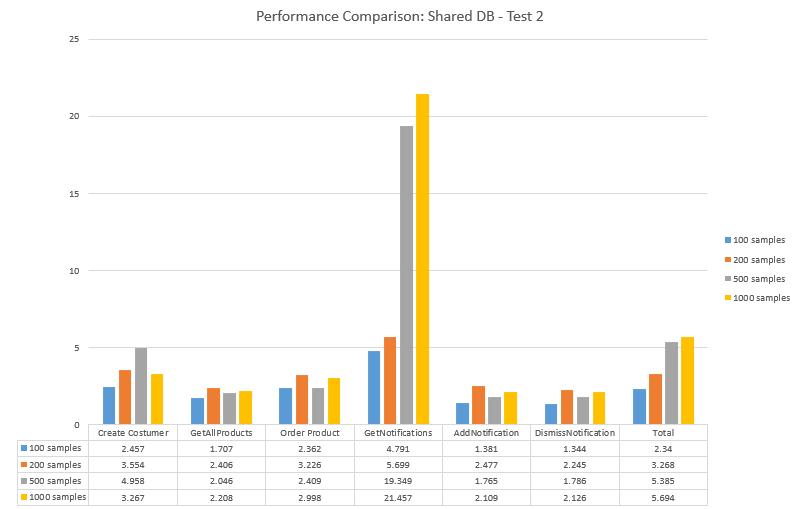
\includegraphics[scale=0.60]{Test_Results/test_2_shared_DB.PNG}
\caption{Test 2 - Shared Database}
\label{fig:test_2_shared_DB}
\end{figure}

\begin{figure}[h!]
\centering
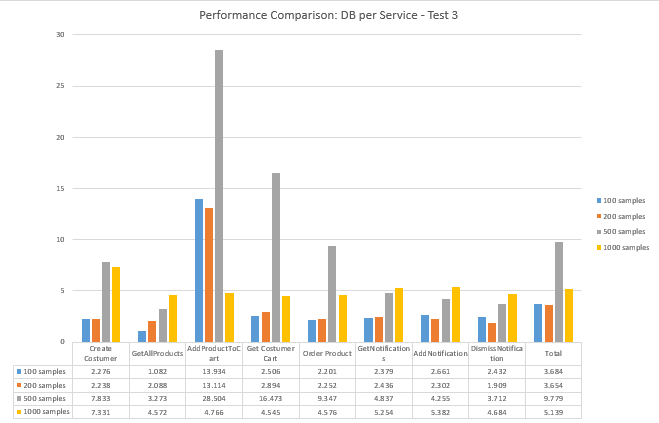
\includegraphics[scale=0.65]{Test_Results/test_3_DB_per_Service.PNG}
\caption{Test 3 - DB per Service}
\label{fig:test_3_DB_per_Service}
\end{figure}

\pagebreak

\begin{figure}[h!]
\centering
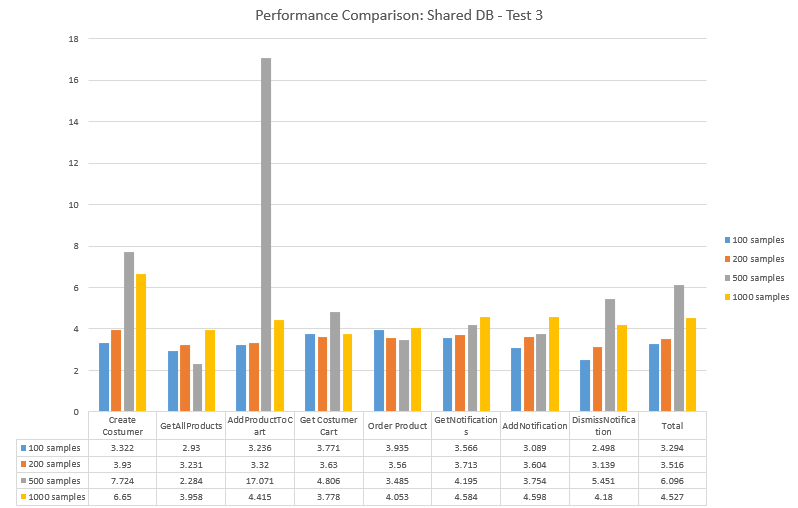
\includegraphics[scale=0.55]{Test_Results/test_3_shared_DB.PNG}
\caption{Test 3 - Shared Database}
\label{fig:test_3_shared_DB}
\end{figure}

\begin{figure}[h!]
\centering
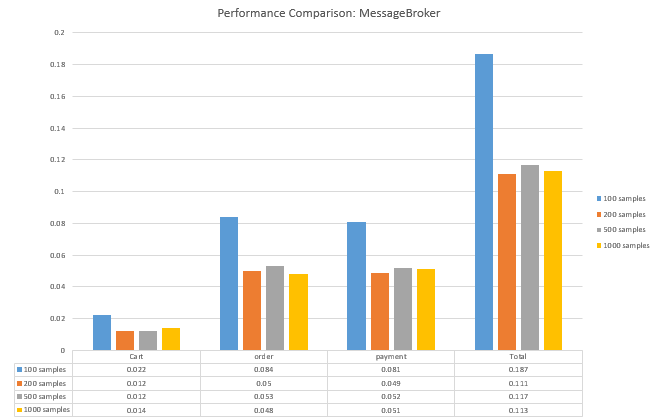
\includegraphics[scale=0.65]{Test_Results/test_MessageBroker.PNG}
\caption{Test - Message Broker Pattern}
\label{fig:test_MessageBroker}
\end{figure}

\pagebreak

\subsection{Discussion of the results}
The test results are a good portrait of the system behaviour. Each prototype is tested with 100, 200, 500 and 1000 samples. It is found that there has been an effect of computer hardware and performance of operating system on the outputs. Nevertheless, it is clear that the performance of the first and second prototypes become worse, when they are tested with a higher number of samples. Additionally, it is observed that when an error occurs while testing, it has a significantly slowing effect on the performance. In the graphs \ref{fig:test_3_DB_per_Service} and \ref{fig:test_3_shared_DB}, it is clearly shown that when executing "add product to cart" operation, errors occurred in the system and the execution time was badly affected by it.
\bigbreak

\noindent In the notification service, all current notifications are saved with their non- permanent IDs in the memory. This implementation’s influence has been detected as a delay on the test results. As shown in figure \ref{fig:test_2_DB_per_Service} and \ref{fig:test_2_shared_DB}, the average response time for getting all current notifications is greater than all other requests’ average response time. When the number of samples are increased, the response time escalates accordingly.

\bigbreak
\noindent Another fact is that in order to add a new costumer, the service needs to access to database and execute insert into query. In the results, it is shown that this request takes more time when comparing with adding a new order request. The main difference in the implementation is that database transaction happens inside of the order service. For example, as shown in the figure \ref{fig:test_2_DB_per_Service}, the request for creating a costumer for 1000 samples takes 12.65 s while the request for ordering products for 1000 samples takes 9 s.

\bigbreak
\noindent Finally, message broker pattern is used in the third prototype and its effect on increasing performance is noticeable \ref{fig:test_MessageBroker}. The cart service, order service and payment service are communicating via a messaging bus and in comparison with other prototypes,  they do not directly communicate with each other. In this model, the asynchronous communication is used and services do not have to wait for a response anymore. This is the main reason of the increased performance.  

\pagebreak

\section{Conclusion}
In conclusion, all patterns used in this project have their benefits and drawbacks. However, it can be seen in the results that using an event-based communication for the microservices allows faster responses as compared to using direct communication between services. Even though database per service and shared database applications' internal structure are similar, their performances differ as a result of using different database architectures. In database per service, to be able to add a product to an order, it needs to join operation to both product service's and order service's databases. Meanwhile in shared database, it is enough to join these two tables. Therefore in this project, unlike the usual, shared database prototype works faster than database per service prototype. 

\section{Future Work}
For the future work, it would be more convenient to use NoSQL databases for the order and product services to avoid using join operations in order to save all products inside of one order. In this particular case, it would be a better choice to use multi index feature of NoSQL databases so that all the product IDs can be saved inside of an array in the database. This array feature doesn't exist in MySQL. With this feature, it will be enough to call the products from one database instead of communicating with two databases to get product information. This service will be separated from others. Moreover, to have a better and faster design, indexes can be created in the SQL database systems. Another point open for development is that implementation details of the web shop application can be improved to make the application more usable in real life.


\pagebreak

\listoffigures
\pagebreak


\bibliographystyle{plain}
\bibliography{references}
\end{document}
